%lägg till theoretical analysis href
\subsection{Design strategy and theoretical analysis}
As mentioned in section \ref{section:purpose}, theoretical analysis is necessary in order to properly evaluate drawbacks, advantages, constraints and requirements of each approach. The analysis is based purely on previous experiments, theoretical facts and information from trusted sources on the Internet, as well as the relevant literature. 

The outcome of this analysis was evaluated in order to find the best combination of features. This combination acted as a specification sheet for building the hybrid centralized application, which is based on a client-server concept, but has some additional blockchain-specific features to improve the system's general performance and usability. The specification sheet was used as a reference throughout the implementation process. The point of merging some aspects from both implementation strategies was to resolve typical drawbacks, which are associated with using a traditional centralized approach, and therefore improve the centralized system, by applying some concepts from decentralized system. The design strategy is illustrated in figure \ref{fig:flowdesign}.

\begin{figure}[H]
\centering
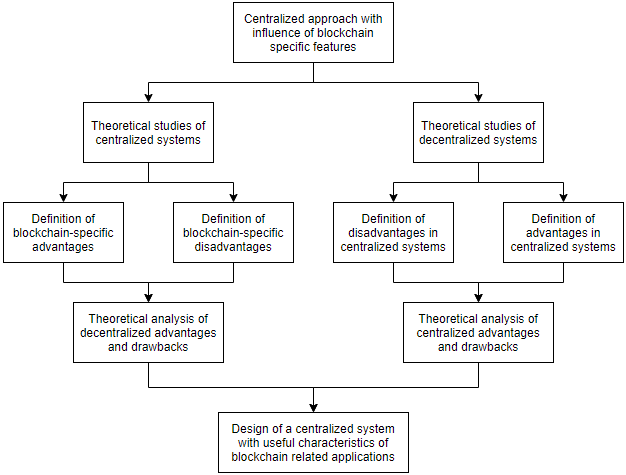
\includegraphics[scale=0.7]{images/designflowchart.png}
\caption{Design strategy and reasoning.}
\label{fig:flowdesign}
\end{figure}

